\graphicspath{{images/}}
\section*{Kellerautomaten}

\begin{remark}
    KA auf englisch: PDA = Push Down Automat
\end{remark}

\begin{definition}{Kellerautomaten}(KA) besitzt «Speicher»

    Deterministischer KA (DKA): $M=\left(Q, \Sigma, \boldsymbol{\Gamma}, \boldsymbol{\delta}, q_{0}, \$, F\right)$
    
    \begin{minipage}{0.4\linewidth}
        $Q$: Menge von Zuständen

        $\Sigma$: Alphabet der Eingabe

        $\Gamma$: Alphabet des Kellers
    \end{minipage}
    \begin{minipage}{0.6\linewidth}
        $q_{0} \in Q$: Anfangszustand

        $\$ \in \Gamma$: Symbol vom Alphabet des Kellers

        $F \subseteq Q$: Akzeptierende Zustände
    \end{minipage}

    Übergangsfunktion: $\boldsymbol{\delta}: \boldsymbol{Q} \times(\boldsymbol{\Sigma} \cup \boldsymbol{\varepsilon}) \times \boldsymbol{\Gamma} \rightarrow \boldsymbol{Q} \times \Gamma^{*}$

    \vspace{1mm}

    \textcolor{pink}{NKA:} $\delta: Q \times(\Sigma \cup \varepsilon) \times \Gamma \rightarrow P(Q \times \Gamma *)$ (Nichtdeterministischer KA)
\end{definition}

\begin{concept}{Übergangsfunktion KA}
    $\forall$ Zustand $q$ und $\forall$ Symbole $x, b$ gilt:
    
    wenn $\delta(q, b, c)$ definiert ist, dann ist $\delta(q, \varepsilon, x)$ undefiniert.

    \vspace*{1mm}

    Darstellung Übergang $\delta(q, b, c)=(p, \omega)$: \emph{$\quad q -b, c / \omega \longrightarrow p$}
\end{concept}

\begin{formula}{Berechnungsschritt}$\delta(q, b, c)=(p, \omega)$ wird wie folgt interpretiert:
    
    \begin{minipage}{0.45\linewidth}
            $q=$ Aktueller Zustand

            $b=$ gelesene Eingabe

            $c=$ entfernt von Stack (pop)
    \end{minipage}
    \begin{minipage}{0.55\linewidth}
            $\omega=$ aktueller Stack + $\omega$ (push)
            \\neustes Symbol zuerst

            $p=$ Neuer Zustand
    \end{minipage}

    {\small (q, b, c) wird als Konfiguration bezeichnet}
\end{formula}

\begin{definition}{Sprache $L(M)$} eines Kellerautomaten $M$ ist definiert durch

    \resizebox{\linewidth}{!}{
    $
    L(M)=\left\{\omega \in \Sigma^{*} \mid\left(q_{0}, \omega, \$\right) \vdash^{*}(q, \varepsilon, \gamma) \text { für ein } q \in F \text { und ein } \gamma \in \Gamma^{*}\right\}
    $
    }
    Elemente von $L(M)$ werden von $M$ akzeptierte Wörter genannt.
\end{definition}

\begin{remark}
    Damit $w_x$ akzeptiert wird, muss $b = \varepsilon$ sein (Stack muss nicht leer sein)
\end{remark}

\begin{KR}{Kellerautomat für kontextfreie Sprache} $\left\{0^{n} 1^{n} \mid n>0\right\}$
    
    \begin{minipage}{0.5\linewidth}
        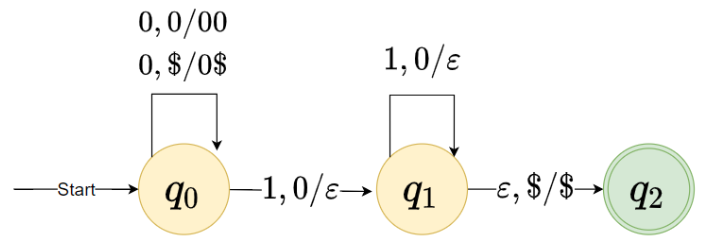
\includegraphics[width=1\linewidth]{images/kellerautomat_sprache.png}
    \end{minipage}
    \begin{minipage}{0.5\linewidth}
        $\omega_{1}=011:$

        \resizebox{\linewidth}{!}{
        $(q_{0}, 011, \$) \vdash(q_{1}, 11,0 \$) \vdash(q_{1}, 1, \$)$}
        $\rightarrow \omega_{1}$ verwerfend 
        
        Das Zeichen \$ zeigt an, dass der «Stack» leer ist.
    \end{minipage}
\end{KR}

\begin{remark}
    Eine Sprache ist kontextfrei, wenn sie von einem NKA akzeptiert wird (nicht unbedingt von DKA).
    Wenn von DKA erkannt, dann ist die Sprache eindeutig.
\end{remark}

\begin{minipage}{0.4\linewidth}
    \begin{concept}{NKA}$\{\omega \omega^{R} \mid \omega \in\{0,1\}^{*}\}$
    \end{concept}
\end{minipage}
\begin{minipage}{0.6\linewidth}
        \includegraphics[width=1\linewidth]{images/nka_übergangsfunktion.png}
\end{minipage}


\begin{example2}{NKA/DKA erkennbar?}
    $L_1 = \{0^n1^n0^n \mid n \in \N\}$, $\sigma = \{0,1\} \rightarrow$ nein

    $L_2 = \{waw^R \mid w \in \{0,1\}^*\}$, $\sigma = \{0,1,a\} \rightarrow$ ja (DKA)

    $L_3 = \{ww \mid w \in \{0,1\}^*\}$, $\sigma = \{0,1\} \rightarrow$ nein
\end{example2}

